\documentclass[12pt,a4paper]{article}
\usepackage[utf8]{inputenc} 
\usepackage{amsmath}
\usepackage{amsthm}
\usepackage{amssymb}
\usepackage{fullpage}
\usepackage{graphicx}

\begin{document}

\title{Retour sur l'AG appliqué à la NLO}

\author{Dumez Dorian}

\maketitle

\section{Implémentation de l'AG}
\begin{itemize}
\item
J'ai étudié la fonction de Rosenbrock en 2 dimension: $100(y - x^2)^2 + (x-1)^2$
\item
Pour le codage des variables j'ai choisis deux codages binaires : chacune des coordonnés du point est représenté par un codage binaire précis à $10^{-6}$
\item
La fonction de fitness est la valeur de la fonction de rRosenbrock en ce point, en effet on souhaite minimiser cette fonction
\item
La procédure de sélection est une roulette. La probabilité de sélection d'une variable est inversement proportionnelle à sa valeur (on remarque que tout est alors normalisé sur le max de la population).
\item
L'opérateur de crossover utilisé est un crossover à un point bi-parental. Ce dernier est effectué séparément sur les deux coordonnés. C'est à dire que chaque coordonné est traité séparément avec un point de croisement différent. Le point de croisement est tiré aléatoirement selon une loi uniforme sur la taille de la chaîne de bit.
\item
L'opérateur de mutation est l'inversion d'un bit. Quand cet opérateur est utilisé il effectue, indépendamment, une négation sur un bit du codage binaire de chaque coordonné. Le bit à inverser est tiré aléatoirement selon une loi uniforme sur la taille de la chaîne de bit.
\item
Le système de population est générationnel, toute la population est mise à jour d'un seul coup, aucun élitisme n'est effectué. Et la sélection vis à vis des parents est faite par tournois.
\item
Le critère d’arrêt est un nombre de génération.
\end{itemize}

\section{Réglages}
\begin{itemize}
\item
La taille de la population est fixé à 350
\item
Le nombre de génération est de 50
\item
La probabilité de crossover est de 1
\item
La probabilité de mutation est de 0.6
\end{itemize}

\newpage

\section{Expérimentations}
\begin{figure}[h]
	\centering
	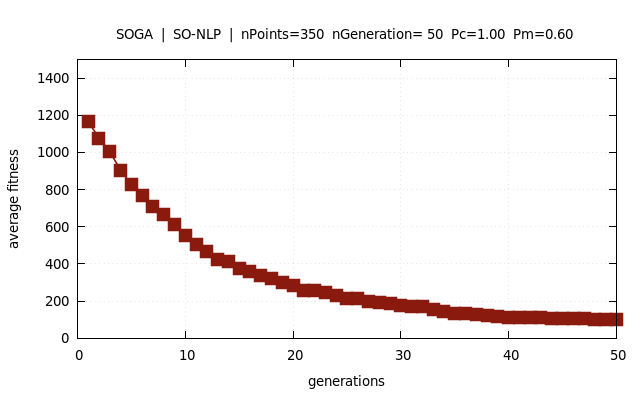
\includegraphics[scale=0.6]{resultat}
	\label{resultat}
	\caption{moyenne de la valeur de la fonction sur la population}
\end{figure}

\begin{figure}[h!]
	\centering
	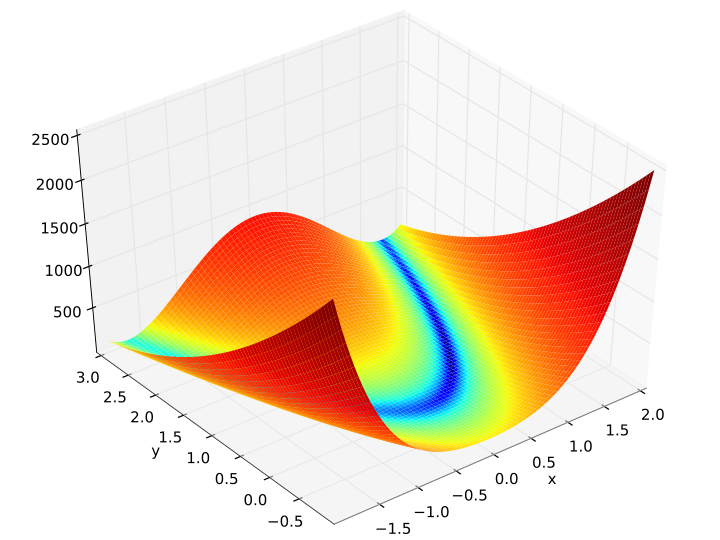
\includegraphics[scale=0.5]{rosenbrock}
	\label{rosenbrock}
	\caption{fonction de rosenbrock}
\end{figure}

\newpage

La moyenne de la la population reste très mauvaise car, au vu de ses réglages, l'algorithme fait peu exploitation. En effet j'ai mis l’accent sur l'exploration car autrement la fonction se bloquai dès qu'elle tombait dans la "rivière". Ainsi la population est très dispensé donc peu progresser le long de la rivière pour trouver des points intéressant. Le meilleur point trouvé est alors $(-0.001 , -0.003 )$ qui a pour valeur $1.004$ alors que le minimum de la fonction est en $(1 , 1)$ avec pour valeur $0$.\\

Mais cette politique d'exploration oblige, pour fonctionner correctement, une grande population pour couvrir asse de terrain ainsi que du temps, d'où les 50 générations. Ces réglages permettent donc d'explorer efficacement l'espace de recherche en recherchant autour des points qui sembles intéressants, sans y rester bloqué.\\

Je suis arrivé vers ses réglages de manière empirique en modifiant les probabilités de crossover et de mutation, puis en cherchant la de taille de population qui leur permettant de s'exprimer au mieux avant de chercher le nombre de génération avant lequel la population se met à stagner.
On remarque alors que ces observations sont en concordance avec la remarque faite sur cette fonction : la rivière est facile à trouver mais la convergence vers le minimum est difficile.\\

Pour conclure on soulignera tout de même que cette fonction possède de bonnes propriétés car c'est un polynôme. Donc des méthodes d'optimisation non linéaire telle que des gradients conjugué fouissent de bien meilleure solution plus rapidement.\\

Au vus de ces remarques j'ai essayé d'initialiser les valeurs des probabilités de mutation et de crossover à des valeurs permettant plus exploitation, pour trouver la rivière, avant de passer après un certains nombre de génération, à des réglages d'explorations comme précédemment. Mais même en jouant un peu avec je n'ai as réussi à améliorer la solution avec cette méthode. 

\end{document}
